% master file siminos/froehlich/slice/FrCv11.tex    pdflatex FrCv11
% $Author: predrag $ $Date: 2010-11-17 08:30:53 -0500 (Wed, 17 Nov 2010) $

                        %% logical setup, no need to edit %%%%%%%%%%
                        \newif\ifpaper \newif\ifPDF               %%
                        \newif\ifboyscout  \newif\ifarticle       %%
                        \boyscouttrue %% commented, WWW/boyscouts %%
                        \articletrue 							  %%
                        \paperfalse\PDFtrue %% hyperlinked    %%%%%%
    % Toggle between draft and non-draft versions
%\boyscoutfalse                 % public, for hyperlinked ChaosBook/projects
%\papertrue\boyscoutfalse     % article for submission

%%   based on edits of aiptemplate.tex AIP REVTeX4 Ver. 4.1, 9 Oct 2009.
% Predrag, created the first draft				2010-11-21

\listfiles
\documentclass[%
 reprint,%					2-column
%secnumarabic,%
 amssymb, amsmath,% ,amsfonts
 aip,cha,% 					Chaos journal
 graphicx
%groupedaddress,%
%frontmatterverbose,
]{revtex4-1}
%\documentclass[aip,cha,graphicx]{revtex4-1}
%\documentclass[aip,reprint]{revtex4-1}

%\draft %obsolete, invoke option instead
% marks overfull lines with a black rule on the right

\usepackage[pdftex]{graphicx}
\usepackage[pdftex,colorlinks]{hyperref}
%\usepackage{array}
\input ../../inputs/editsDasbuch   %% editing comments, DasBuch style
\input def            %% edited, initially from dasbuch/book/inputs/def.tex
\input ../../inputs/defsFroehlich     %% all Stefan edits: \renewcommand, etc
\graphicspath{{../../figs/}{../../Fig/}}  %% directories with color graphics files
\hypersetup{
   pdfauthor=Stefan Froehlich and Predrag Cvitanovic,
   pdfkeywords=complex Lorenz flow,
   pdftitle=Reducing continuous symmetries}

\begin{document}
\title{Reduction of continuous symmetries by the method of slices}

% repeat the \author .. \affiliation  etc. as needed
% \email, \thanks, \homepage, \altaffiliation all apply to the current author.
% Explanatory text should go in the []'s,
% actual e-mail address or url should go in the {}'s for \email and \homepage.
% Please use the appropriate macro for the type of information

% \affiliation command applies to all authors since the last \affiliation command.
% The \affiliation command should follow the other information.

\author{Stefan Froehlich}
%\email[]{Your e-mail address}
%\thanks{}
%\altaffiliation{}
%\affiliation{}

\author{Predrag Cvitanovi\'{c}}
\email[]{predrag@gatech.edu}
%\homepage[]{Your web page}
%\thanks{}
\affiliation{Center for Nonlinear Science,
        School of Physics, Georgia Institute of Technology,
        Atlanta, GA 30332-0430}

\date{\today}

\begin{abstract}
% insert abstract here
\end{abstract}

\pacs{
02.20.-a, 05.45.-a, 05.45.Jn, 47.27.ed
% 02.20.-a  Group theory, mathematics
% 05.45.-a 	Nonlinear dynamics and chaos
% 05.45.Jn 	High-dimensional chaos
% 47.10.Fg 	Dynamical systems methods (in Fluid Mechanics)
% 47.27.ed 	Dynamical systems approaches (turbulent flows)
% 47.52.+j 	Chaos in fluid dynamics
	}

\maketitle %must follow title, authors, abstract and \pacs

% If in two-column mode, this environment will change to single-column format so that long equations can be displayed.
% Use only when necessary.
%\begin{widetext}
%$$\mbox{put long equation here}$$
%\end{widetext}

% \begin{figure}
% \includegraphics{}%
% \caption{\label{}}%
% \end{figure}

% Tables may be be put in the text as floats.
% Here is an example of the general form of a table:
% Fill in the caption in the braces of the \caption{} command. Put the label
% that you will use with \ref{} command in the braces of the \label{} command.
% Insert the column specifiers (l, r, c, d, etc.) in the empty braces of the
% \begin{tabular}{} command.
%
% \begin{table}
% \caption{\label{} }
% \begin{tabular}{}
% \end{tabular}
% \end{table}

\section{Introduction}
\label{sec:intro}

Suppose you are observing turbulence in a pipe flow. Here you see a
pattern, and there you see a pattern that seems much like the first one.
How ``much like the first one?'' If the dynamics of the system under study is invariant under
a group of continuous symmetries, one way of answering the question is by
measuring distances between different states in the
symmetry-reduced \statesp\ $\pS/\Group$, a space in which each group orbit (class
of physically equivalent states) is represented by a single point.
But there exist no preferred, one-size fits all
symmetry-reduction method. The literature
(see \refrefs{CBcontinuous,SiCvi10,SiminosThesis} for a review) broadly
offers two approaches (a) Hilbert invariant polynomial bases, and (b) methods which
slice group orbits much in the way that \Poincare\ sections cut across
time-evolving trajectories. The invariant polynomial approaches can use
the symmetries to recast

This paper describes  the question in a


\Mslices\ as applied to chaotic/turbulent dynamics has been
studied in \refrefs{SiminosThesis,SiCvi10,Wilczak09,CBcontinuous}.

The new results of this paper are:

\section{\Mslices}
\label{sec:mslices}
Suppose you are observing turbulence in a pipe flow, or your
defibrillator has a mesh of sensors measuring electrical currents that
cross your heart, or you have a precomputed pattern, and are sifting
through the data set of observed patterns for something like it. Here you see a
pattern, and there you see a pattern that seems much like the first one.
How ``much like the first one?''
Think of the first pattern (represented
by a point {\slicep} in the \statesp\  \pS) as a
`template'\rf{rowley_reconstruction_2000,rowley_reduction_2003} or a
`reference state' and use the symmetries of the flow to slide and rotate
the `template' until it overlays the second pattern
(a point $\ssp$ in the \statesp), \ie, act with elements of
the symmetry group \Group\ on the template ${\slicep} \to
{\LieEl}{\slicep}$ until the distance between the two patterns
\beq
|\ssp - {\LieEl}{\slicep}|
    = |\sspRed - \slicep|
    \label{minDistance0}
\eeq
is minimized. Here $\sspRed$ is the point on the group orbit
of $\ssp$,
\beq
\ssp=\LieEl \sspRed
	\qquad
\LieEl \in \Group
\,,
\ee{sspOrbit}
closest to the template {\slicep}, where we shall measure distance
$|\ssp|^2=\braket{\ssp}{\ssp}$ in terms of the Euclidian inner product
\( %beq
\braket{x}{y} = \sum_i^d {x}_i y_i
%    \,,\; %\qquad
% x, y \in \pS \subset \reals^d
	\,,
\) %\ee{innerR}
or, if the \statesp\ is a normed function space,
\( %\beq
\braket{g}{f} = \int dx \, \dual{g}(x) f(x)
\,,
\) %\ee{innerL2}
with the associated $L^2$ norm $|f|^2 = \braket{f}{f}$.
In practice, we always represent such functions by discrete
meshes or truncated basis sets, with a (possibly large)
finite-dimensional \statesp\  $\pS \subset \reals^d$.

If we parameterize a Lie group element $\LieEl=\LieEl(\gSpace)$ by
parameters $\gSpace = (\gSpace_1,\gSpace_2,\cdots\gSpace_N)$, the minimal
distance satisfies the extremum conditions
\beq
0  =
\frac{\partial ~~}{\partial \gSpace_a} |\ssp - \LieEl\slicep|^2
   =
\braket{\sspRed - \slicep}{\sliceTan{a}}
    \,,\qquad
	  \sliceTan{a} = \Lg_a \slicep
\,.
\label{PCsectQ}
\eeq

More explicitly, an element of a compact Lie group that is continuously
connected to the identity can be expressed as
\beq
\LieEl(\gSpace)=e^{{\gSpace} \cdot \Lg }
    \,,\qquad
\gSpace \cdot \Lg = \sum_{a=1}^N \gSpace_a \Lg_a
\,.
\ee{FiniteRot}
The group action parameters $\gSpace_a$ are often referred to as
``phases,'' or ``shifts.''
The group orbit of a point $\ssp$ under the group $\Group$ is the set of all
points that $\ssp$ is mapped to under the groups actions
\beq
\pS_\ssp=\{{g} \, \ssp: g \in \Group\}.
\ee{GroupOrbit}
As \Group\ is a symmetry of the system, the
length $|\ssp|$ is invariant under symmetry operations, $\Group \subset \On{d}$
and the Lie algebra {generators} $\Lg_a$ are a set of $N$ linearly
independent $[d\!\times\!d]$ antisymmetric matrices acting linearly on
the {\statesp} vectors $\ssp \in \pS \subset \reals^d$. An infinitesimal
% , $|\delta \gSpace| \ll 1$,
group action is generated by
$
\LieEl(\delta \gSpace) \simeq 1 + \delta \gSpace \cdot \Lg
\,.
$ %\ee{eq:infinitesimal}
A transformation induced by an infinitesimal
time-dependent variation of group `phases'
$\delta \gSpace_a = \timeStep \, \dot{\gSpace_a}$ is
\beq
\dot{\ssp} = \dot{\gSpace} \cdot \groupTan(\ssp)
\,,
\ee{PC:groupTan1}
where
\beq
 \groupTan_{a}(\ssp) = \Lg _{a} \ssp
    \,,\qquad
 a=1,2,\cdots,N,
\ee{PC:groupTan}
is the group action tangent at $\ssp$.
So $\dot{\gSpace} \cdot \groupTan(\ssp)$ is the velocity
of the flow along the group orbit of \ssp.
We use $\groupTan_a(\ssp)$ notation (rather than
$\Lg_{a}\ssp$) to emphasize that the group action
induces a \emph{tangent field} at $\sspRed$.


{\bf Slice:}
The minimum distance condition \refeq{minDistance0} together with
Euclidean norm says that the
closest point $\sspRed$ in the group orbit of \statesp\ point $\ssp$ lies in a
$(d\!-\!N)$-dimensional hyperplane defined by \refeq{PCsectQ},
a hyperplane through the template point $\slicep$,
normal to the group action tangent
space $\sliceTan{}$.
This hyperplane is called a `slice' and is an example of
symmetry reduction by transverse sections of
group orbits\rf{FelsOlver98,FelsOlver99,OlverInv} that
can be traced back to Cartan's \mframes\rf{CartanMF}.

As a generic group orbit is a curved $N$-dimensional manifold embedded in
the \statesp, several values of $\gSpace$ might be local extrema of the
distance function \refeq{PCsectQ}. For example, group orbits of \SOn{2}\
are topologically circles, and the distance function \refeq{minDistance0}
has maxima, minima and inflection points as extrema. We only care about
those that are local {\em minima}, for which all the eigenvalues of the
symmetric matrix $[N\!\times\!N]$ matrix of second derivatives of
distance,
\beq
\frac{\partial^2}
     {\partial \gSpace_a \partial \gSpace_b}
        |\sspRed - \slicep|^2
    =
%  - \braket{\Lg_a e^{\gSpace \cdot \Lg} \ssp}{\sliceTan{b}}=
  - \braket{\groupTan_a(\sspRed)}{\sliceTan{b}}=
  \braket{\sspRed}{\Lg_a \Lg_b\slicep}
\ee{PCinflPoint}
are positive.

$\Lg_a \Lg_b$ plays a fundamental role in the theory of Lie groups.
Any representation of a compact group $\Group$ is fully
reducible, and for a Lie group
the invariant tensors constructed by contractions
of $\Lg_a$ are useful for identifying irreducible
representations. The simplest such invariant is
\beq
\dual{\Lg} \cdot \Lg = \sum_\alpha C_2^{(\alpha)} \, \id^{(\alpha)}
\,,
\ee{QuadCasimir}
where $C_2^{(\alpha)}$ is the quadratic Casimir for
irreducible representation labeled $\alpha$, and
$\id^{(\alpha)}$ is the identity on the $\alpha$-irreducible
subspace, 0 elsewhere. $ C_2^{(\alpha)} =0$ if $\alpha$
is an invariant subspace.
The dot product of two tangent fields in
\refeq{PCinflPoint} is thus a sum of inner products
weighted by Casimirs,
\beq
\braket{\groupTan(\sspRed)}{\groupTan(\slicep)}
   = \sum_\alpha C_2^{(\alpha)} \dual{\sspRed}_i\, \delta_{ij}^{(\alpha)} \slicep_j
\,.
\ee{braket}
An example is the Fourier series \refeq{tangL2norm}.
For compact groups $C_2^{(\alpha)}$ are strictly nonnegative by
the antihermiticity \refeq{antiHerm} of Lie algebra generators.


The physically most interesting minimum is
presumably the closest one, the absolute minimum of \refeq{minDistance0}.
It does not matter whether the group is compact, for example $\SOn{n}$, or
noncompact, for example the Euclidean group $E_2$ that underlies the generation
of spiral patterns\rf{Barkley94}; in either case any group orbit has
one or several locally closest passages to the template state.







If the two patterns are
close, their group orbits will be nearly parallel, and for a smooth flow
the slice will be transverse to all group orbits of $\ssp$ in a
neighborhood of \slicep.

%    \PC{recycle this:
%{\em {\mslices}}
%    }


By the antihermiticity of $\Lg$, \refeq{antiHerm},  we have
$\braket{\slicep}{\sliceTan{a}}=0$, and the transformation parameters
$\gSpace$ for which the state $\ssp$ is closest to the template
$\slicep$ are fixed by $N$ slice conditions
\beq
\braket{\sspRed}{\sliceTan{a}} =0
    \,,\qquad
\sspRed = \LieEl(\gSpace) \ssp
\,.
\ee{PCsectQ0}

A given compact group orbit intersects a slice at least twice, and
possibly many times, so we need a prescription for how to
pick a unique \reducedsp\ point as the representative of the entire group
orbit.


However, we will be bolder, and show next that for a generic template
$\slicep$ (\ie, any $\slicep$ whose group orbit is $N$-dimensional), the
slice hyperplane \refeq{PCsectQ} cuts across the group orbit of {\em
every} point in the full \statesp\ \pS.





The distance surface $|\sspRed - \slicep|$ can have inflection points,
What role do they play? They are non-generic, but if we consider distance
to local minima at successive instants of a time-evolving trajectory,
coalescence of
nearby minima, maxima pairs cannot be avoided. At the instant of
coalescence the denominator in \refeq{SF:sliceEas} goes through a simple
pole, and the integrated trajectory within slice might jump.



\subsection{}
\subsubsection{}


\section{Dynamics in the slice}
\label{sect:MovFrameODE}


 \begin{figure}
 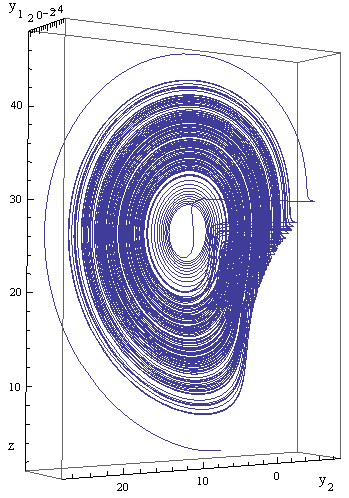
\includegraphics[width=0.35\textwidth]{CLEreduced}%
 \caption{\label{fig:CLErx2y1z}
A $\{y_1,y_2,z\}$ plot of the \reducedsp\ \cLf\ strange attractor
with initial point
%$(x_1, x_2, y_1, y_2, z) = (1, 2, 3, 1, 2)$
in the
slice normal to $\sliceTan{}=(1,0,0,0,0)$. Contrast this plot with
\reffig{fig:CLEx2y1z}, and note the apparent discontinuities in the
reduced flow.
 }%
 \end{figure}

\subsection{Traversing a slice singularity}
\label{sect:passingSing}

 \begin{figure}
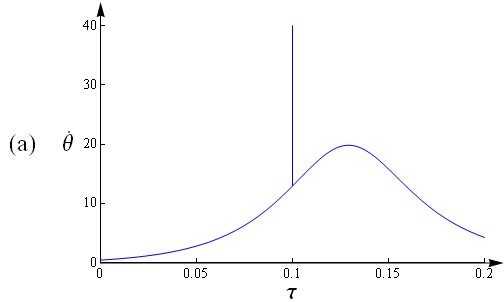
\includegraphics[width=0.45\textwidth]{CLEsingpass}
\\
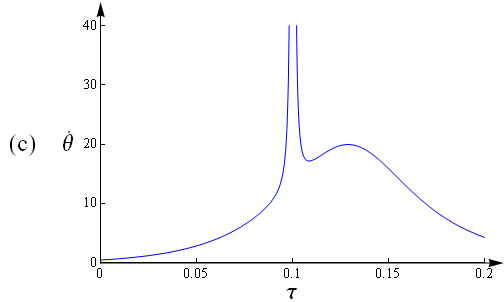
\includegraphics[width=0.45\textwidth]{CLEnearsing2}%
 \caption{\label{fig:dthetasing}
 (a) $\dot{\gSpace}$ of the trajectory with initial point
$\ssp_0=(-1.22, 3.212, -4.31, 1.11, 4)$ as it passes through a
singularity at $t=0.1$ in the slice with slice fixing point
$\slicep=(0.782,-0.277,-0.4,0.12,0)$.
(b) $\dot{\gSpace}$ of the trajectory with initial point $\ssp_0+\delta
\ssp$ where $\delta\ssp=(0.01,0,0,0,0)$.
 }%
 \end{figure}

\section{Conclusion}
\label{sec:intro}

\input concl

\begin{acknowledgments}
Authors are grateful to
D.~Barkley,
W.-J.~Beyn,
K.A.~Mitchell,
B.~Sandstede,
R.~Wilczak,
and in particular E.~Siminos and R.L.~Davidchack
for many spirited exchanges.
S.F. work was supported by the National Science Foundation
grant DMR~0820054 and a Georgia Tech President's Undergraduate
Research Award.
P.C. thanks Glen Robinson Jr. for support. 	
\end{acknowledgments}

% Create the reference section using BibTeX:
\bibliography{../../bibtex/siminos}

\end{document}
%
% ****** End of file aiptemplate.tex ******
